\documentclass[eng]{csam}
\usepackage{graphicx}
\usepackage{natbib}
\usepackage{amsmath,multirow}
\usepackage{enumerate,array}
\usepackage{xcolor}
\usepackage[ruled,vlined]{algorithm2e}
\usepackage{multirow}
\usepackage{kotex}

\def \bY { \mathbf{ Y } }
\def \bX { \mathbf{ X } }
\def \bU { \mathbf{ U } }
\def \bmu { \boldsymbol{ \mu } }
\def \bSigma { \boldsymbol{ \Sigma } } 
\def \bphi { \boldsymbol{ \phi } }
\def \bepsilon { \boldsymbol{ \epsilon } }
\def \bD { \boldsymbol{\mathcal{D}} }

%% ==================================================================
%% Templete File for Communications of the Korean Statistical Society
%% Korean Statistical Society (office@kss.or.kr)
%% ==================================================================

%%\submit{draft}
% ==================== Do not Modify here ============================
\submit{final}
\volumn{20}{1}{2013}
\receive{0000}{00}{00} \revise{0000}{00}{00}  \accept{0000}{00}{00}
\setpagenum{1}
% ====================================================================


\heading{Bootstrap aggregated classification for sparse functional data}{Hyunsung Kim, Yaeji Lim}

\begin{document}

\title{Bootstrap aggregated classification for sparse functional data}

\author{Hyunsung Kim\address[a]{Department of Statistics, Chung-Ang University, Korea}, 
	Yaeji Lim\footnote{Corresponding author: Professor, Department of Applied Statistics, Chung-Ang University, 84 Heukseok-ro, Dongjak-gu, Seoul 06974, Korea. E-mail: yaeji.lim@gmail.com}\address[b]{Department of Applied Statistics, Chung-Ang University, Korea}}

\begin{abstract}
	{\color{red}
		Abstract
	}
\end{abstract}

\keywords{functional principal component analysis, bootstrap aggregating, classification, sparse data}

\section{Introduction}
{\color{red} 
	Prior studies
	
	Description of sections
}


\section{Preliminaries}
Functional data analysis (FDA) is a kind of statistics that analyzes the curves or functions rather than single points. In FDA, data (or curve) is defined on the infinite dimension, so dimensionality reduction becomes a key issue. One of the popular dimension reduction method in FDA is functional principal component analysis (FPCA) which finds directions of the variation and exploits by data-driven basis called functional principal component (FPC) scores. 

\subsection{Functional principal compnent analysis}
%Let $X(t)$ is a square integrable random process for $t \in \mathcal{T}$ with mean function $\mu(t) = E\big(X(t)\big)$ and covariance function $G(s,t) = \text{cov}\big(X(s),X(t)\big)$ for $s, t \in \mathcal{T}$.
Let $X(t)$, defined on finite $\mathcal{T}$, is a square integrable random process which means $X(\cdot) \in L_2(\mathcal{T})$ with mean function $\mu(t) = E\big[X(t)\big]$ and covariance function $G(s,t) = \text{cov}\big[X(s),X(t)\big]$ for $s, t \in \mathcal{T}$. By Mercer's theorem, the covariance function can be represented as $G(s,t) = \sum_{k=1}^\infty \lambda_k \phi_k(s) \phi_k(t)$ where $\lambda_1 \ge \lambda_2 \ge \dots \ge 0 $ are non-negative eigenvalues satisfying $\sum_{k=1}^\infty \lambda_k < \infty$ and $\phi_k$'s are the corresponding orthonormal eigenfunctions. By the $K$-truncated Karhunen-Lo\`{e}ve expansion, the $i$th random curve can be represented as
\begin{equation*}
	X_i(t) = \mu(t) + \sum_{k=1}^K \xi_{ik} \phi_k(t), \hspace{0.5cm} t \in \mathcal{T}
\end{equation*}
where $K$ is the number of basis functions, and $\xi_{ik} = \int_{\mathcal{T}} \big( X_i(t) - \mu(t) \big)\phi_k(t) dt $ are uncorrelated variables with mean 0 and variance $\lambda_k$.
%$E(\xi_{ik}) = 0$, $E(\xi_{ij} \xi_{ik}) = 0$ for $j \ne k$, and $E(\xi_{ik}^2) = \lambda_k$.

In the real world, each curve is often observed with measurement errors. Then the $i$th curve with random noise is denoted as
\begin{equation*}
	U_i(t) = X_i(t) + \epsilon_i(t), \hspace{0.5cm} t \in \mathcal{T}
\end{equation*}
where $\epsilon_i(t)$ are the uncorrelated measurement errors with mean 0 and variance $\sigma^2$.

The number of basis functions, $K$, is often selected by proportion of variance explained (PVE). Yao {\em et al.} (2005) presented AIC that is more efficient in computation than cross-validation. Li {\em et al.} (2013) proposed BIC and proved its consistency on FPCA.



\subsection{Functional principal component analysis for sparse functional data}
When each curve is observed at sparse or irregular time points, we can't apply above method directly. The covariance function can't be computed easily and also estimated FPC scores by numerical integration be biased. So, James {\em et al.} (2001) proposed the reduced rank model based on the mixed effects model and estimate FPC function and scores by EM algorithm. Yao {\em et al.} (2005) proposed principal component analysis through conditional expectation (PACE) method to obtain the unbiased FPC scores.

Let $t_{ij} \in \mathcal{T}$ is the $j$th time point observed in the $i$th curve $X_i(\cdot)$ where $i = 1, 2, \dots, n$, $j = 1, 2, \dots, n_i$.
Then, the $i$th curve for sparse functional data using from $K$-truncated FPCA can be expressed as
\begin{equation*}
	%\bY_i = \bmu_i + \sum_{k=1}^\infty \xi_{ik} \bphi_{ik} + \bepsilon_i.
	U_i(t_{ij}) = \mu(t_{ij}) + \sum_{k=1}^K \xi_{ik} \phi_k(t_{ij}) + \epsilon_i(t_{ij}), \hspace{0.5cm} t_{ij} \in \mathcal{T}
\end{equation*}
where $K$ is the number of basis functions, and $\epsilon_i(t_{ij})$ are the random noises.

Let $i$th curve $\bX_i = \big( X_i(t_{i1}), \dots, X_i(t_{in_i}) \big)^T$, $i$th curve with measurment error $\bU_i = \big( U_i(t_{in_1}), \dots, U_i(t_{in_i}) \big)^T$, the mean function $\bmu_i = \big( \mu(t_{i1}), \dots, \mu(t_{in_i}) \big)^T$, the FPC functions $\bphi_{ik} = \big( \phi_k(t_{i1}), \dots, \phi_k(t_{in_i}) \big)^T$, and the measurment errors $\bepsilon_i = \big( \epsilon_i(t_{i1}), \dots, \epsilon_i(t_{in_i}) \big)^T$.
The best linear unbiased prediction (BLUP) of $\xi_{ik}$, $k$th FPC scores of $i$th subject, by PACE is
\begin{equation*}
	\tilde \xi_{ik} = E[\xi_{ik} \vert \bU_i] = \lambda_k \bphi_{ik}^T\bSigma_{\bU_i}^{-1}(\bU_i - \bmu_i),
\end{equation*}
where $\bSigma_{\bU_i} = \text{cov}(\bU_i, \bU_i) = \text{cov}(\bX_i, \bX_i) + \sigma^2\mathbf{I}_{n_i}$,

From the above, the PACE estimate of $\xi_{ik}$ is obtained as follow
\begin{equation*}
	\hat \xi_{ik} = \widehat E[\xi_{ik} \vert \bU_i] = \hat\lambda_k \hat\bphi_{ik}^T \widehat\bSigma_{\bU_i}^{-1}(\bU_i - \hat\bmu_i).
\end{equation*}
where $\widehat\bSigma_{\bU_i} = \widehat{\text{cov}}(\bU_i, \bU_i) = \widehat{\text{cov}}(\bX_i, \bX_i) + \hat\sigma^2\mathbf{I}_{n_i}$.


{\color{red}
	How to apply FPCA for sparse data?
}




\section{Method (Functional classifier ensemble)}
\subsection{Functional classification(Classification based on functional principal component scores)}
For classification, functional generalized linear model (FGLM) was proposed by James (2002) and Müller \& Stadtmüller (2005).

Let $\bX_i = X_i(\cdot)$ is the $i$th curve, $Y_i$ is its response, $\beta(\cdot)$ is the coefficient function, and $g(\cdot)$ is a link function. Denote $\mu = E(Y_i | \bX_i)$, then, the functional generalized linear model (FGLM) is
\begin{align*}
	g(\mu) &= \alpha + \int_{\mathcal{T}} \beta(t) X_i(t) dt \\
	       &= \alpha + \sum_{t \in \mathcal{T}} \beta(t) X_i(t).
\end{align*}

Since we can only observe $X_i(t)$ at a finite time points, the integral can be substituted with a summation. But it has a problem that the estimate of $\beta(\cdot)$ may be unstable since $\beta(\cdot)$ be an extremely high dimensional vector.

We can solve this problem by expanding $\beta(\cdot)$ in terms of a set of basis functions. If FPCA is performed, we can also use data-driven orthonormal basis functions to represent $\beta(\cdot)$. In addition, it is stable because most of the variation can be expressed in a small number, $K$.

Denote $X_i(t) = \sum_{k=1}^K \xi_{ik} \phi_k(t)$ and $\beta(t) = \sum_{k=1}^K \beta_k \phi_k(t)$ from $K$-truncated FPCA model, then the FGLM is represented as
\begin{equation*}
	g(\mu) = \alpha + \sum_{k=1}^K \beta_k \xi_{ik}.
\end{equation*}

If we set $g(\cdot)$ as logit link, the FGLM above becomes functional logistic regression for binary classification problems. Therefore, we can construct the functional classifier by modeling a conventional classifier on FPC scores.



\subsection{Bootstrap aggregating}
Bootstrap aggregating (Bagging) is the ensemble method using bootstrap ideas proposed by Breiman (1996). It is a method of extracting samples several times with replacement and learning each model to aggregate results. It can avoid overfitting problems and also reduce its variance. 
Generally, it is aggregated into an average in regression problems, and a majority vote in classification problems.
%In classification problem that the response variable is categorical, it is generally aggregated as a majority vote.

\subsubsection{Majority vote}
Suppose there are $g$ response classes with $C_1, \dots, C_g$, and a classifier, $\hat f^{(b)}(x)$ for $b=1, \dots, B$, obtained from $b$th bootstrap resample. Then, the estimate of bagged classifier by the majority vote is
\begin{equation*}
\hat y_{\text{bag}} = \arg\max_j \# \big\{ b \mid \hat f^{(b)}(x) = C_j \big\}.
\end{equation*}

\subsubsection{Out-of-bag accuracy weighted vote}


\subsection{Bootstrap aggregated functional classifier with sparse FPCA}
We propose the method that aggregate independent functional classifiers from bootstrap resamples. For dimension reduction, FPCA with PACE is performed for each functional classifier.


Suppose we have $n$ curves, $\bU_1, \dots, \bU_n$ observed at sparse and irregular time points. Also, we have the response variable $y_1,\dots,y_n$ with $g$ different class labels for each curve. Denote the set of sparse $n$ curves as $\bD = \left\{ \left( \bU_i, y_i \right) \mid i=1, \dots, n \right\}$ and $\bD^{(b)} = \left\{ \left( \bU^{(b)}_i, y^{(b)}_i \right) \bigm| i=1, \dots, n \right\}$ for $b=1,\dots,B$ is a bootstrap resample from $\bD$. For each bootstrap functional data, we perform FPCA with PACE approach. First $K$ FPC scores are chosen by the appropriate criterian, PVE, BIC, cross-validation, etc. In this paper, we select $K$ satisfiying PVE is greater than 0.99. Using these $K$ FPC scores, we construct a classifier, like support vector machine (SVM), linear discriminant analysis (LDA), quadratic discriminant analysis (QDA), etc. Then, we can get $B$ classifiers from each bootstrap sample. When we observe a new curve, we can obtain $B$ predictions from $B$ classifiers and aggregate it by majority vote. Then, we can get the prediction from bagged classifier with sparse FPCA. The summary of procedure is shown in the below algorithm.

\begin{algorithm}[H]
	\caption{Bagged functional classifier with sparse FPCA}
	\begin{enumerate}
		\item For $b = 1, \dots, B$, repeat
		\begin{enumerate}
			\item Generate a bootstrap resample $\bD^{(b)}$ from the data $\bD$.
			\item Perform functional principal component analysis for $\bD^{(b)}$.
			\item Estimate the FPC scores by PACE.
			\item Select $K$, the number of FPCs, such that PVE $\ge 0.99$.
			\item Construct a classifier on $K$ FPC scores.
		\end{enumerate}
%		\item Given a new curve $\bU^*$, obtain each $B$ predictions from above $B$ classifiers.
		\item Given a new curve $\bU^*$, for $b = 1, \dots, B$, repeat
		\begin{enumerate}
			\item Estimate the FPC scores by PACE using FPC function from $\bD_{b}$.
			\item Obtain the prediction $\hat y^{(b)}$ from above $b$th classifiers.
		\end{enumerate}
	
		\item From $\hat y^{(1)}, \dots, \hat y^{(B)}$, obtain the final prediction $\hat y_{bag}$ aggreated by majority vote.
	\end{enumerate}
\end{algorithm}

{\color{red}
	algorithm flow image??
}



\section{Simulation studies}

\subsection{Simulation 1}
In this simulation, we consider 3 situations, (A) different mean and variance, (B) different mean, and (C) different variance.

We generate a total of $n=200$ curves with 2 classes ($n/2$ for each class) from $U_{gi}(t) = \mu_g(t) + \sum_{k=1}^3 \xi_{gk} \phi_k(t) + \epsilon_i(t)$ for $g = 0, 1$ and $t \in [0, 10]$. The FPC functions are $\phi_k(t) = \cos(\pi kt /5) / \sqrt{5}$ for $k$ is odds and $\phi_k(t) = \sin(\pi kt /5) / \sqrt{5}$ for $k$ is even. In Table 1, the parameters of mean and variance are decided for each models. The mean functions $\mu_g(t)$ are generated for each class and the FPC scores $\xi_{gk}$ are sampled from $i.i.d. \ N(0, \lambda_{gk})$ for $k=1,2,3$. The measurement error $\epsilon_i(t)$ is sampled from $i.i.d. \ N(0, 0.5^2)$ To make each curve sparse, the number of grids for $i$th curve $n_i$ is randomly selected from 5 to 10, and the observed time points $t_{ij}$, $j=1, \dots, n_i$, are selected from $i.i.d. \ Uniform(0, 10)$.

To compare the proposed method with single functional classifier, we randomly split the generated data to training and test set with 100 each. We consider 7 classification models (logistic regression, SVM with linear kernel, SVM with gaussian kernel, LDA, QDA and naive bayes), and the truncation number $K$ is selected to satisfy PVE $\ge 0.99$ in FPCA. We compute percentage of classification error and standard error for 100 Monte Carlo repetitions for each classifier.
\textcolor{red}{앞에서 SVM, LDA, QDA 언급 필요}



%The total of 6 models, logistic regression, SVM with linear kernel, SVM with gaussian kernel, LDA, QDA and naive bayes were performed. 
%
%In this study, we compare the performances of different classifiers (logistic regression, support vector machine, linear discriminant analysis, quadratic discriminant analysis, naive bayes).

\begin{table}[ht]
	\footnotesize
	\centering
	\caption{The parameters of 3 different models from simulation 1}
	\tabcolsep=11.5pt
	\begin{tabular}{cccc}
		\hline \hline
		Model & $g$ & $\mu_g(t)$ & $\boldsymbol\lambda_g$ \\ 
		\hline
		\multirow{2}{*}{A} & 0 & $t + \sin(t)$ & $(4, 2, 1)$ \\
		                   & 1 & $t + \cos(t)$ & $(16, 8, 4)$ \\
		\hline
		\multirow{2}{*}{B} & 0 & $t + \sin(t)$ & $(4, 2, 1)$ \\
						   & 1 & $t + \cos(t)$ & $(4, 2, 1)$ \\
		\hline
		\multirow{2}{*}{C} & 0 & $t + \sin(t)$ & $(4, 2, 1)$ \\
		                   & 1 & $t + \sin(t)$ & $(16, 8, 4)$ \\
		\hline \hline
	\end{tabular}
\end{table}

Shown in Table 2, \textcolor{red}{결과 언급}

%\begin{table}[ht]
%	\footnotesize
%	\centering
%	\caption{The average classification error with standard error in percentage from 100 Monte Carlo repetitions for 3 different simulation designs}
%	\tabcolsep=6.5pt
%%	\tiny
%	\begin{tabular}{cccccccc}
%		\hline\hline
%			  &        & Logistic   & SVM      & SVM        &     &     & Naive \\
%		Model & Method & Regression & (Linear) & (Gaussian) & LDA & QDA & Bayes \\ 
%		\hline
%		\multirow{3}{*}{A} & Single        & 17.60 (4.84) & 17.48 (5.12) & 15.28 (5.30) & 17.07 (4.74) & 15.07 (4.82) & 16.48 (4.55) \\ 
%					       & Majority vote & 15.47 (4.23) & 15.66 (4.41) & 13.16 (4.35) & 15.53 (4.08) & 13.63 (4.17) & 15.23 (4.09) \\ 
%						   & OOB weight    & 16.14 (4.25) & 16.32 (4.49) & 13.85 (4.34) & 16.30 (4.17) & 14.20 (4.12) & 15.71 (3.97) \\ 
%		\hline
%		\multirow{3}{*}{B} & Single        & 11.88 (3.43) & 11.45 (3.49) & 12.00 (4.25) & 11.25 (3.55) & 12.85 (3.62) & 13.97 (4.39) \\ 
%						   & Majority vote & 10.70 (3.29) & 10.44 (3.13) & 10.96 (3.70) & 10.44 (3.24) & 11.59 (3.36) & 12.41 (3.38) \\ 
%						   & OOB weight    & 11.39 (3.27) & 11.21 (3.00) & 11.75 (3.60) & 11.05 (3.30) & 12.32 (3.36) & 13.07 (3.59) \\ 
%		\hline
%		\multirow{3}{*}{C} & Single        & 50.49 (5.65) & 49.53 (5.47) & 32.79 (5.03) & 50.59 (5.63) & 31.20 (4.51) & 30.50 (4.71) \\
%						   & Majority vote & 49.45 (5.58) & 48.25 (6.15) & 31.27 (5.09) & 49.50 (5.68) & 30.76 (4.06) & 29.80 (4.29) \\ 
%						   & OOB weight    & 48.85 (5.53) & 47.83 (6.03) & 31.51 (5.13) & 48.81 (5.47) & 31.01 (4.03) & 30.11 (4.25) \\ 
%		\hline\hline
%	\end{tabular}
%\end{table}


\begin{table}[ht]
	\footnotesize
%	\centering
	\caption{The average classification error with standard error in percentage from 100 Monte Carlo repetitions for 3 different simulation designs with different class proportion}
	\tabcolsep=4.5pt
	%	\tiny
	\begin{tabular}{cccrrrrrr}
		\hline\hline
		      &          &        & \multicolumn{1}{c}{Logistic} & \multicolumn{1}{c}{SVM} & \multicolumn{1}{c}{SVM} & & & \multicolumn{1}{c}{Naive} \\
		Model & $P(C_1)$ & Method & \multicolumn{1}{c}{Regression} & \multicolumn{1}{c}{(Linear)} & \multicolumn{1}{c}{(Gaussian)} & \multicolumn{1}{c}{LDA} & \multicolumn{1}{c}{QDA} & \multicolumn{1}{c}{Bayes} \\ 
		\hline
		\multirow{12}{*}{A} & \multirow{3}{*}{0.5} & Single        & 17.60 (4.84) & 17.48 (5.12) & 15.28 (5.30) & 17.07 (4.74) & 15.07 (4.82) & 16.48 (4.55) \\ 
						    &					  & Majority vote & 15.47 (4.23) & 15.66 (4.41) & 13.16 (4.35) & 15.53 (4.08) & 13.63 (4.17) & 15.23 (4.09) \\ 
						    &					  & OOB weight    & 16.14 (4.25) & 16.32 (4.49) & 13.85 (4.34) & 16.30 (4.17) & 14.20 (4.12) & 15.71 (3.97) \\ 
		\cline{2-9}
		& \multirow{3}{*}{0.4} & Single        & 17.65 (4.91) & 17.71 (5.27) & 15.75 (5.84) & 17.72 (4.98) & 15.19 (4.82) & 16.31 (4.78) \\
		&					   & Majority vote & 15.68 (4.02) & 15.56 (4.00) & 13.74 (4.58) & 15.39 (3.97) & 14.50 (4.68) & 15.51 (4.44) \\ 
		&					   & OOB weight    & 16.24 (3.77) & 16.33 (3.90) & 14.49 (4.22) & 16.13 (3.85) & 15.07 (4.57) & 15.95 (4.41) \\ 
		
		\cline{2-9}
		&\multirow{3}{*}{0.3} & Single        & 17.26 (5.50) & 17.87 (6.12) & 15.21 (5.57) & 17.17 (5.32) & 14.89 (5.24) & 15.23 (5.04) \\
		&      				  & Majority vote & 15.90 (4.35) & 16.40 (5.31) & 13.25 (4.67) & 15.97 (4.17) & 14.64 (4.24) & 14.98 (4.14) \\ 
		&					  & OOB weight    & 16.71 (4.19) & 17.34 (5.14) & 14.15 (4.68) & 16.87 (3.95) & 15.37 (4.23) & 15.72 (4.38) \\ 
		\cline{2-9}
		&\multirow{3}{*}{0.2} & Single        & 15.60 (4.31) & 16.31 (4.31) & 14.32 (4.92) & 15.45 (4.31) & 13.55 (4.51) & 13.91 (4.12) \\ 
		&					  & Majority vote & 14.19 (4.14) & 15.12 (4.70) & 12.80 (4.61) & 14.04 (3.91) & 13.92 (3.88) & 13.70 (3.99) \\ 
		&					  & OOB weight    & 15.26 (4.20) & 16.31 (5.00) & 14.01 (4.67) & 15.08 (3.96) & 15.02 (4.03) & 14.81 (4.03) \\ 
		\hline
\multirow{12}{*}{B} & \multirow{3}{*}{0.5} & Single        & 11.88 (3.43) & 11.45 (3.49) & 12.00 (4.25) & 11.25 (3.55) & 12.85 (3.62) & 13.97 (4.39) \\ 
&					  & Majority vote & 10.70 (3.29) & 10.44 (3.13) & 10.96 (3.70) & 10.44 (3.24) & 11.59 (3.36) & 12.41 (3.38) \\ 
&					  & OOB weight    & 11.39 (3.27) & 11.21 (3.00) & 11.75 (3.60) & 11.05 (3.30) & 12.32 (3.36) & 13.07 (3.59) \\ 
\cline{2-9}
& \multirow{3}{*}{0.4} & Single        & 11.13 (3.49) & 10.99 (3.38) & 11.93 (3.78) & 10.84 (3.4) & 12.11 (3.62) & 13.72 (4.21) \\
&					   & Majority vote & 9.96 (2.88) & 9.81 (2.58) & 10.73 (3.25) & 9.74 (2.79) & 10.82 (3.15) & 11.95 (3.33) \\
&					   & OOB weight    & 10.85 (2.92) & 10.64 (2.79) & 11.53 (3.27) & 10.63 (2.92) & 11.74 (3.26) & 12.73 (3.56) \\ 

\cline{2-9}
&\multirow{3}{*}{0.3} & Single        & 10.23 (3.55) & 10.28 (3.51) & 11.10 (3.77) &  9.62 (3.22) & 11.33 (3.44) & 12.33 (3.43) \\
&      				  & Majority vote &  9.35 (3.29) &  9.39 (3.16) &  9.62 (2.95) &  9.07 (2.82) & 10.31 (3.01) & 10.93 (3.01) \\ 
&					  & OOB weight    & 10.36 (3.46) & 10.45 (3.33) & 10.69 (3.26) & 10.17 (2.99) & 11.29 (3.27) & 12.00 (3.21) \\ 
\cline{2-9}
&\multirow{3}{*}{0.2} & Single        & 9.61 (2.98) & 9.14 (2.79) & 9.54 (3.65) & 8.82 (2.89) & 10.63 (3.86) & 10.65 (3.43) \\ 
&					  & Majority vote & 8.41 (2.68) & 8.21 (2.46) & 8.30 (2.66) & 7.81 (2.55) &  9.37 (3.07) &  9.30 (2.85) \\ 
&					  & OOB weight    & 9.67 (2.93) & 9.57 (2.74) & 9.61 (2.87) & 9.15 (2.86) & 10.60 (3.31) & 10.64 (3.15) \\ 
\hline
\multirow{12}{*}{C} & \multirow{3}{*}{0.5} & Single        & 50.49 (5.65) & 49.53 (5.47) & 32.79 (5.03) & 50.59 (5.63) & 31.20 (4.51) & 30.50 (4.71) \\
&					  & Majority vote & 49.45 (5.58) & 48.25 (6.15) & 31.27 (5.09) & 49.50 (5.68) & 30.76 (4.06) & 29.80 (4.29) \\ 
&					  & OOB weight    & 48.85 (5.53) & 47.83 (6.03) & 31.51 (5.13) & 48.81 (5.47) & 31.01 (4.03) & 30.11 (4.25) \\ 
\cline{2-9}
& \multirow{3}{*}{0.4} & Single        & 47.78 (4.25) & 41.04 (4.32) & 33.24 (5.06) & 47.55 (4.17) & 31.12 (4.61) & 30.04 (4.47) \\ 
&					   & Majority vote & 47.23 (4.39) & 40.78 (3.51) & 32.71 (4.90) & 47.14 (4.54) & 30.71 (4.25) & 29.42 (4.04) \\
&					   & OOB weight    & 47.56 (4.65) & 41.12 (3.63) & 33.22 (4.76) & 47.43 (4.59) & 31.06 (4.08) & 29.78 (4.01) \\ 

\cline{2-9}
&\multirow{3}{*}{0.3} & Single        & 33.58 (3.97) & 30.09 (3.36) & 29.61 (4.00) & 33.26 (3.77) & 27.49 (4.33) & 26.85 (4.01) \\ 
&      				  & Majority vote & 33.19 (4.02) & 30.09 (3.36) & 28.96 (3.91) & 32.91 (3.78) & 26.95 (3.87) & 26.44 (3.82) \\ 
&					  & OOB weight    & 33.93 (4.20) & 30.79 (3.51) & 29.78 (4.00) & 33.62 (3.94) & 27.91 (3.85) & 27.19 (3.61) \\ 
\cline{2-9}
&\multirow{3}{*}{0.2} & Single        & 21.06 (2.91) & 19.65 (2.67) & 20.26 (3.19) & 20.86 (2.75) & 21.31 (3.45) & 21.01 (3.2) \\ 
&					  & Majority vote & 20.64 (2.78) & 19.65 (2.67) & 19.93 (2.89) & 20.54 (2.85) & 20.09 (2.85) & 20.52 (2.65) \\
&					  & OOB weight    & 21.79 (3.12) & 20.77 (3.00) & 21.10 (3.23) & 21.69 (3.19) & 21.42 (3.16) & 21.77 (3.01) \\
		\hline\hline
	\end{tabular}
	OOB weight = Out-of-bag weighted vote
\end{table}



%\begin{table}[ht]
%	\footnotesize
%	\centering
%	\caption{The simulation design of 3 different models from simulation 1}
%	\tabcolsep=11.5pt
%	\begin{tabular}{ccccc}
%		\hline \hline
%		Model & $\mu_0(t)$ & $\mu_1(t)$ & $\boldsymbol\lambda_0$ & $\boldsymbol\lambda_1$ \\ 
%		\hline
%		A & $t + \sin(t)$ & $t + \cos(t)$ & $(4, 2, 1)$ & $(16, 8, 4)$ \\
%		B & $t + \sin(t)$ & $t + \cos(t)$ & $(4, 2, 1)$ & $(4, 2, 1)$ \\
%		C & $t + \sin(t)$ & $t + \sin(t)$ & $(4, 2, 1)$ & $(16, 8, 4)$ \\
%		\hline \hline
%	\end{tabular}
%\end{table}


\subsection{Simulation 2}
In second simulation, we refer the procedure of generating data from Yao {\em et al.} (2016). 
\begin{align*}
	\text{Model A: } & f(x) = \exp(\langle \beta_1, X \rangle / 2) - 1, \\
	\text{Model B: } & f(x) = \arctan(\pi \langle \beta_1, X \rangle) + \exp(\langle \beta_2, X \rangle / 3) - 1, \\
	\text{Model C: } & f(x) = \arctan(\pi \langle \beta_1, X \rangle / 4).
\end{align*}

Shown in Table 3, \textcolor{red}{결과 언급}

{\color{red}
	Data generating
	
	100 Monte Carlo simulation(generate + split)
	
	Result
}

\begin{table}[ht]
	\footnotesize
%	\centering
	\caption{The average classification error with standard error in percentage from 100 Monte Carlo repetitions for 3 different simulation designs}
	\tabcolsep=6.5pt
%	\tiny
	\begin{tabular}{cccccccc}
		\hline\hline
			  &        & Logistic   & SVM      & SVM        &     &     & Naive \\
		Model & Method & Regression & (Linear) & (Gaussian) & LDA & QDA & Bayes \\ 
		\hline
		\multirow{3}{*}{A} & Single        & 16.71 (2.33) & 16.82 (2.20) & 17.50 (2.76) & 16.62 (2.30) & 17.77 (2.56) & 18.41 (2.66) \\
					       & Majority vote & 15.62 (1.95) & 15.86 (1.87) & 16.19 (2.28) & 15.79 (1.96) & 16.51 (2.14) & 17.32 (2.42) \\ 
						   & OOB weight    & 16.00 (2.02) & 16.21 (1.94) & 16.56 (2.28) & 16.14 (1.98) & 16.86 (2.09) & 17.71 (2.43) \\ 
		\hline
		\multirow{3}{*}{B} & Single        & 12.85 (2.41) & 12.79 (2.40) & 13.27 (2.65) & 12.77 (2.40) & 13.83 (2.56) & 14.77 (2.74) \\ 
						   & Majority vote & 11.20 (1.84) & 11.14 (1.89) & 11.54 (1.98) & 11.19 (1.85) & 11.93 (2.03) & 13.29 (2.36) \\ 
						   & OOB weight    & 11.62 (1.86) & 11.54 (1.90) & 11.96 (1.96) & 11.59 (1.86) & 12.33 (2.06) & 13.63 (2.35) \\ 
		\hline
		\multirow{3}{*}{C} & Single        & 14.46 (2.17) & 14.34 (2.18) & 15.27 (2.69) & 14.29 (2.17) & 15.32 (2.36) & 16.05 (2.22) \\
						   & Majority vote & 13.15 (1.73) & 13.14 (1.78) & 13.62 (2.08) & 13.14 (1.82) & 13.78 (1.90) & 14.88 (2.09) \\ 
						   & OOB weight    & 13.53 (1.81) & 13.50 (1.78) & 13.99 (2.03) & 13.52 (1.84) & 14.18 (1.92) & 15.22 (2.12) \\ 
		\hline\hline
	\end{tabular}
	OOB weight = Out-of-bag weighted vote
\end{table}




%\begin{table}[t]
%\footnotesize
%\centering
%\caption{Structure of data.}\label{tb:data1}
%\tabcolsep=35.5pt
%\begin{tabular}{ccccc}
%\hline \hline
%\multirow{2}*{$N$} & \multicolumn{4}{c}{factor level} \\\cline{2-5}
% & 1 & 2 & $\cdots$ & $I$ \\\hline
%1        & $x_{11}$ & $x_{21}$ & $\cdots$ & $x_{I1}$ \\
%2        & $x_{12}$ & $x_{22}$ & $\cdots$ & $x_{I2}$ \\
%$\vdots$ & $\vdots$ & $\vdots$ & $\ddots$ & $\vdots$ \\
%$n$      & $x_{1n}$ & $x_{2n}$ & $\cdots$ & $x_{In}$ \\
%\hline \hline
%\end{tabular}
%\end{table}


\section{Real data analysis}
\subsection{Berkely growth data}
To compare the proposed method with single classifier, we consider the berkely growth data presented in Tuddenham \& Snyder (1954). The dataset was measured height for 93 individuals, 54 girls and 39 boys. There are 31 observations from ages 1 to 18 for each curve. These dense curves with 54 girls and 39 boys are shown in Figure 1.

\begin{figure}[h]
	\centering
	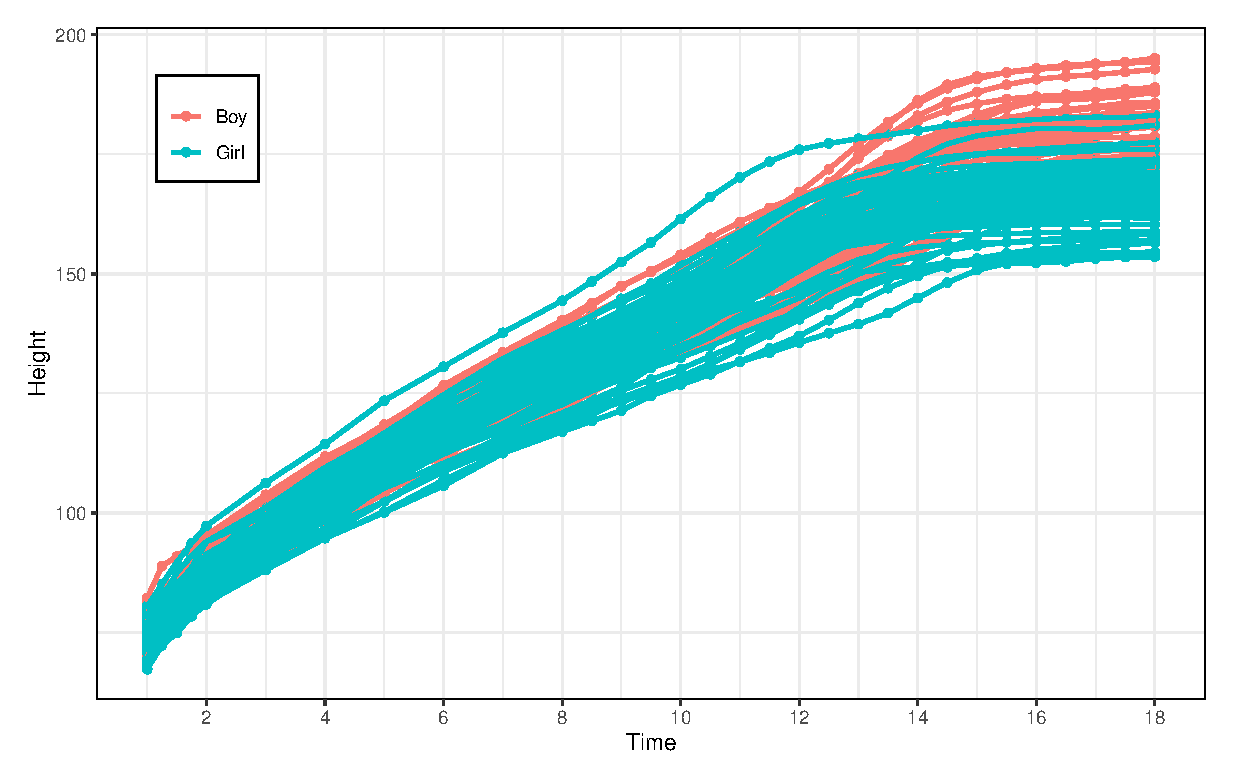
\includegraphics[height=6cm,keepaspectratio=true]{img/growth.eps}
	\caption{The berkely growth data of 93 individuals.}
	\label{fig:rsxb}
\end{figure}

Our method is to apply to sparse data, so we have transformed data into arbitrarily sparse. The number of observation $n_i$ was randomly selected from 12 to 15 and its time points also randomly selected from original time points. We randomly selected 62 curves as training set and the remaining 31 curves as test set.
For these sparse data, we performed the proposed bagged functional classifiers with sparse FPCA and compared to the single classifiers. The total of 6 models, logistic regression, SVM with linear kernel, SVM with gaussian kernel, LDA, QDA and naive bayes were performed. We repeated this process 100 times for different split. There are the average classification error and its standard error in Table 4. All bagged classifiers showed better performances than single models, and bagged QDA showed the best. 

\begin{table}[ht]
	\footnotesize
	\centering
	\caption{The average classification error with standard error in percentage from 100 random split for berkerly growth data}
	\tabcolsep=11.5pt
	\begin{tabular}{ccccccc}
		\hline \hline
	           & Logistic   & SVM      & SVM        &     &     & Naive \\
		Method & Regression & (Linear) & (Gaussian) & LDA & QDA & Bayes \\ 
		\hline
		Single        & 7.3 (4.80) & 5.3 (3.20) & 5.7 (4.03) & 5.8 (3.34) & 5.6 (3.35) & 5.6 (3.90) \\ 
		Majority vote & 5.9 (4.12) & 4.9 (3.19) & 5.3 (3.51) & 5.4 (3.24) & 4.9 (3.57) & 5.5 (3.96) \\ 
		OOB weight    & 5.9 (4.12) & 5.0 (3.22) & 5.4 (3.62) & 5.4 (3.27) & 4.9 (3.54) & 5.5 (3.96) \\ 
		\hline \hline
	\end{tabular}
\end{table}

{\color{red}
	Data description
	
	Result	
}


\subsection{Spinal bone mineral density data}
Second, we consider the sparse functional data, the spinal bone mineral density data presented in Bachrach {\em et al.} (1999). The dataset has the spinal bone mineral density for 280 individuals, 153 females and 127 males measured at sparse and irregualar time points. There are $2 \sim 4$ observations for each curve. The dataset has also ethnicity information such that Asian, Black, Hispanic and White. For this data, we consider gender classification. These sparse curves with 153 females and 127 males are shown in Figure 2.
\begin{figure}[h]
	\centering
	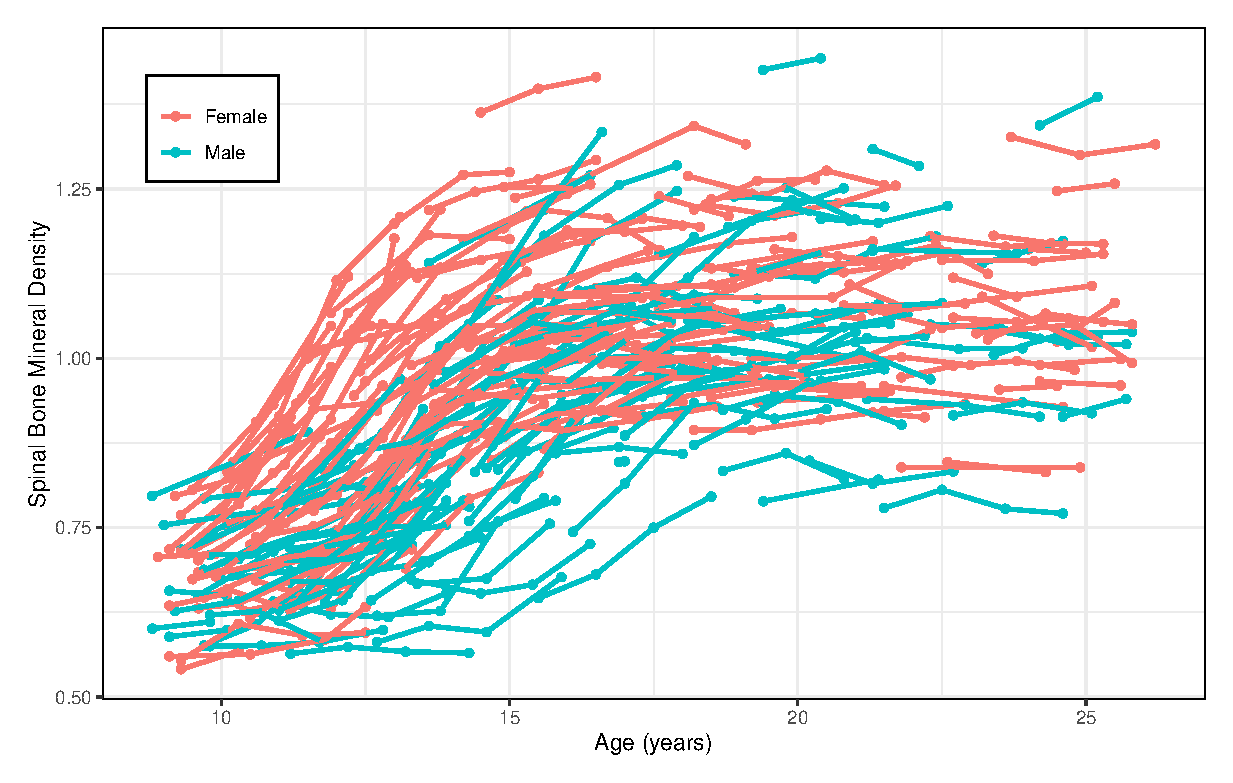
\includegraphics[height=6cm,keepaspectratio=true]{img/spnbmd.eps}
	\caption{The spinal bone mineral density of 280 individuals.}
	\label{fig:rsxb}
\end{figure}

%We try to classify gender for proposed method. First, we split the sparse spinal bone mineral density data to training and test set. We generate 100 bootstrap resamples from training set. We applied FPCA with PACE for each bootstrap resample to obtain the FPC scores. We construct 100 classifiers on FPC scores from each bootstrap resample. From test set, 100 bootstrap predictions are obtained for each curve. Then we get the final prediction by majority vote from 100 bootstrap predictions. We repeat 100 times with different seeds for different split of training and test set. 
We performed the same procedure except to make the data sparse. The data was randomly divided into 187 training and 93 test sets. The same 6 classifiers were considered on the above and both single and bagged classifiers were performed for each classifier. This procedures were applied to 100 different splits. The results are shown in Table 5. The proposed methods showed better performance than single classifiers. The bagged logistic regression with majority vote showed the best performance in this data.

\begin{table}[ht]
	\footnotesize
	\centering
	\caption{The average classification error with standard error in percentage from 100 random split for spinal bone mineral density data}
	\tabcolsep=10.5pt
	\begin{tabular}{ccccccc}
		\hline \hline
			   & Logistic   & SVM      & SVM        &     &     & Naive \\
		Method & Regression & (Linear) & (Gaussian) & LDA & QDA & Bayes \\ 
		\hline
		Single        & 31.3 (4.30) & 32.0 (4.27) & 33.2 (4.71) & 31.4 (4.44) & 33.3 (4.10) & 32.3 (4.33) \\ 
		Majority vote & 30.2 (3.72) & 30.8 (4.18) & 31.2 (3.88) & 30.4 (3.77) & 31.6 (3.78) & 30.9 (3.83) \\ 
		OOB weight    & 30.3 (3.71) & 30.8 (4.07) & 31.4 (3.81) & 30.5 (3.82) & 31.8 (3.71) & 30.9 (3.86) \\ 
		\hline \hline
	\end{tabular}
\end{table}



\section{Conclusion and discussion}
{\color{red}
	conclusion and result	
}




\section*{Acknowledgement}
This research was supported by the Chung-Ang University Graduate Research Scholarship in 2019.

\begin{reference}
	\item[] Bachrach, L. K., Hastie, T., Wang, M. C., Narasimhan, B., \& Marcus, R. (1999). Bone mineral acquisition in healthy Asian, Hispanic, black, and Caucasian youth: a longitudinal study. {\em The journal of clinical endocrinology \& metabolism}, {\bf 84}, 4702-4712.
	\item[] Breiman, L. (1996). Bagging predictors. {\em Machine learning}, {\bf 24}, 123-140.
	%	\item[] Breiman, L. (2001). Random forests. {\em Machine learning}, {\bf 45}, 5-32.
	\item[] Friedman, J., Hastie, T., \& Tibshirani, R. (2001). {\em The elements of statistical learning.}, Springer series in statistics, New York.
	\item[] James, G. M., Hastie, T. J., \& Sugar, C. A. (2000). Principal component models for sparse functional data. {\em Biometrika}, {\bf 87}, 587-602.
	\item[] James, G. M., \& Hastie, T. J. (2001). Functional linear discriminant analysis for irregularly sampled curves. {\em Journal of the Royal Statistical Society: Series B (Statistical Methodology)}, {\bf 63}, 533-550.
	\item[] James, G. M. (2002). Generalized linear models with functional predictors. {\em Journal of the Royal Statistical Society: Series B (Statistical Methodology)}, {\bf 64}, 411-432.
	\item[] Li, Y., Wang, N., \& Carroll, R. J. (2013). Selecting the number of principal components in functional data. {\em Journal of the American Statistical Association}, {\bf 108}, 1284-1294.
	\item[] Müller, H. G., \& Stadtmüller, U. (2005). Generalized functional linear models. {\em the Annals of Statistics}, {\bf 33}, 774-805.
	\item[] Ramsay, J. O., \& Silverman, B. W. {\em Functional Data Analysis}, 2nd ed., Springer Series in Statistics, New York.
	\item[] Tuddenham, R. D., \& Snyder, M. M. (1954). Physical growth of California boys and girls from birth to eighteen years. {\em University of California publications in child development}, {\bf 1}, 183-364.
	\item[] Yao, F., Müller, H. G., \& Wang, J. L. (2005). Functional data analysis for sparse longitudinal data. {\em Journal of the American Statistical Association}, {\bf 100}, 577-590.
	\item[] Yao, F., Wu, Y., \& Zou, J. (2016). Probability-enhanced effective dimension reduction for classifying sparse functional data. {\em Test}, {\bf 25}, 1-22.
	
\end{reference}

%\bibliographystyle{apalike}
%\bibliography{ref}
%\nocite{*}

\end{document}
